%%%%%%%%%%%%%%%%%%%%%%%%%%%%%%%%%%%%%%%%%%%%%%%%%%%%%%%%%%%%%%%%%%%%%%%%%%%%%%%%
%% MASTER'S THESIS                                                            %%
%%                                                                            %% 
%% Title (en): Multi-Agent Systems and Organizations                          %%
%% Title (cs): Multiagentní systémy a organizace                              %%
%%                                                                            %%
%% Author: Bc. Lukáš Kúdela                                                   %%
%% Supervisor: Prof. RNDr. Petr Štěpánek, DrSc.                               %%
%%                                                                            %%
%% Academic year: 2011/2012                                                   %%
%%%%%%%%%%%%%%%%%%%%%%%%%%%%%%%%%%%%%%%%%%%%%%%%%%%%%%%%%%%%%%%%%%%%%%%%%%%%%%%%

\chapter{Agents and Multi-Agent Systems}

% Chapter intro
The purpose of this chapter is to introduce \textit{agents}\comments{FO} and \textit{multi-agent systems}\comments{FO}.
The introduction is kept as short as possible, sticking to the most fundamental characteristics.
Nevertheless, it provides all necessary background to understand the ideas presented in this thesis.

% Agents and MASs - referecnes
% English
A slightly more detailed overview of multi-agent systems can be found in \cite{Wooldridge95} and \cite{Wooldridge02}. A more in-depth (yet still general) introduction \cite{Wooldridge09} has become the \textit{de facto} standard textbook on multi-agent systems.
\cite{Weiss99} is another excellent introduction to multi-agent systems in the context of distributed artificial intelligence.
Alternatively, in \cite{Shoham08} the authors take an algorithmic, game-theoretic and logical\footnote{As in mathematical-logical, not rational.} approach to multi-agent systems.
% Czech
To our knowledge, \cite{Kubik04} is the most complete coverage of multi-agent systems in Czech, while \cite{Kubik03} is an overview by the same author.

%%%%%%%%%%%%%%%%%%%%%%%%%%%%%%%%%%%%%%%%%%%%%%%%%%%%%%%%%%%%%%%%%%%%%%%%%%%%%%%%
\section{Agents}

% No single universally accepted definition of agent exists
Unfortunately, no single and universally accepted definition of an agent exists in the agents community.
However, this does not seem to be a problem at all; despite the lack of agreement on terminological details, many researchers are coming up with interesting agent theories and numerous practitioners are developing useful agent applications.
Still, it is important that at least some definition of an agent exists---if for nothing else, then to protect it from being overused and thus stripped of any meaning.

% Two usages of the term 'agent'
Two usages of the term \textit{agent} can be recognized.
The first is weaker and does not appear to be disputed; the second is stronger and generates more discussion in the community.
In this thesis, it is sufficient to use the weaker notion of agency.

% Agent - definition: situatedness and autonomy
An \textit{agent} is a computational entity that is \textit{situated in an environment} and that is \textit{capable of autonomous action} in this environment in order to meet its design objectives \cite{Wooldridge02}.
% Situatedness
Being situated in an environment means that the agent can \textit{sense} (or \textit{perceive}) it through its \textit{sensors} and \textit{act} upon it through its \textit{actuators} (or \textit{effectors}).
Note that the definition does not specify the \textit{type} of environment an agent inhabits; agents can occupy many different types of environments, for example a physical, virtual or software environment.
% Autonomy
Being capable of autonomous action means that the ``agents are able to act without the intervention of humans or other systems: they have control both over their own internal state, and over their behavior.'' \cite{Wooldridge02}

% Intelligent agent - definition: reactivity, proactivity and social skills
An important type of agent---especially in artificial intelligence---is an \textit{intelligent agent}\comments{FO}.
In \cite{Wooldridge02}, an \textit{intelligent agent} is defined as an agent capable of \textit{flexible} autonomous action in order to meet its design objectives, where flexibility means three things:
\begin{itemize}
	\item \textit{reactiveness}---an ability to respond in a timely fashion to changes that occur in the agent's environment,
	\item \textit{proactiveness}---an ability to exhibit goal-directed behaviour by taking the initiative, and
	\item \textit{social ability}---an ability to interact with other agents (and possibly humans).
\end{itemize}

Figure~\ref{figure:agent-environment-interaction} shows an abstract view of agent interacting with its environment.
The agent obtains \textit{percepts} from the environment as input (using its sensors) and exerts \textit{actions} upon the environment as output (using its actuators).
This interaction is usually an ongoing, non-terminating one.

% Figure: Agent - agent interacting with its environment
\begin{figure}[h]
	\centering
	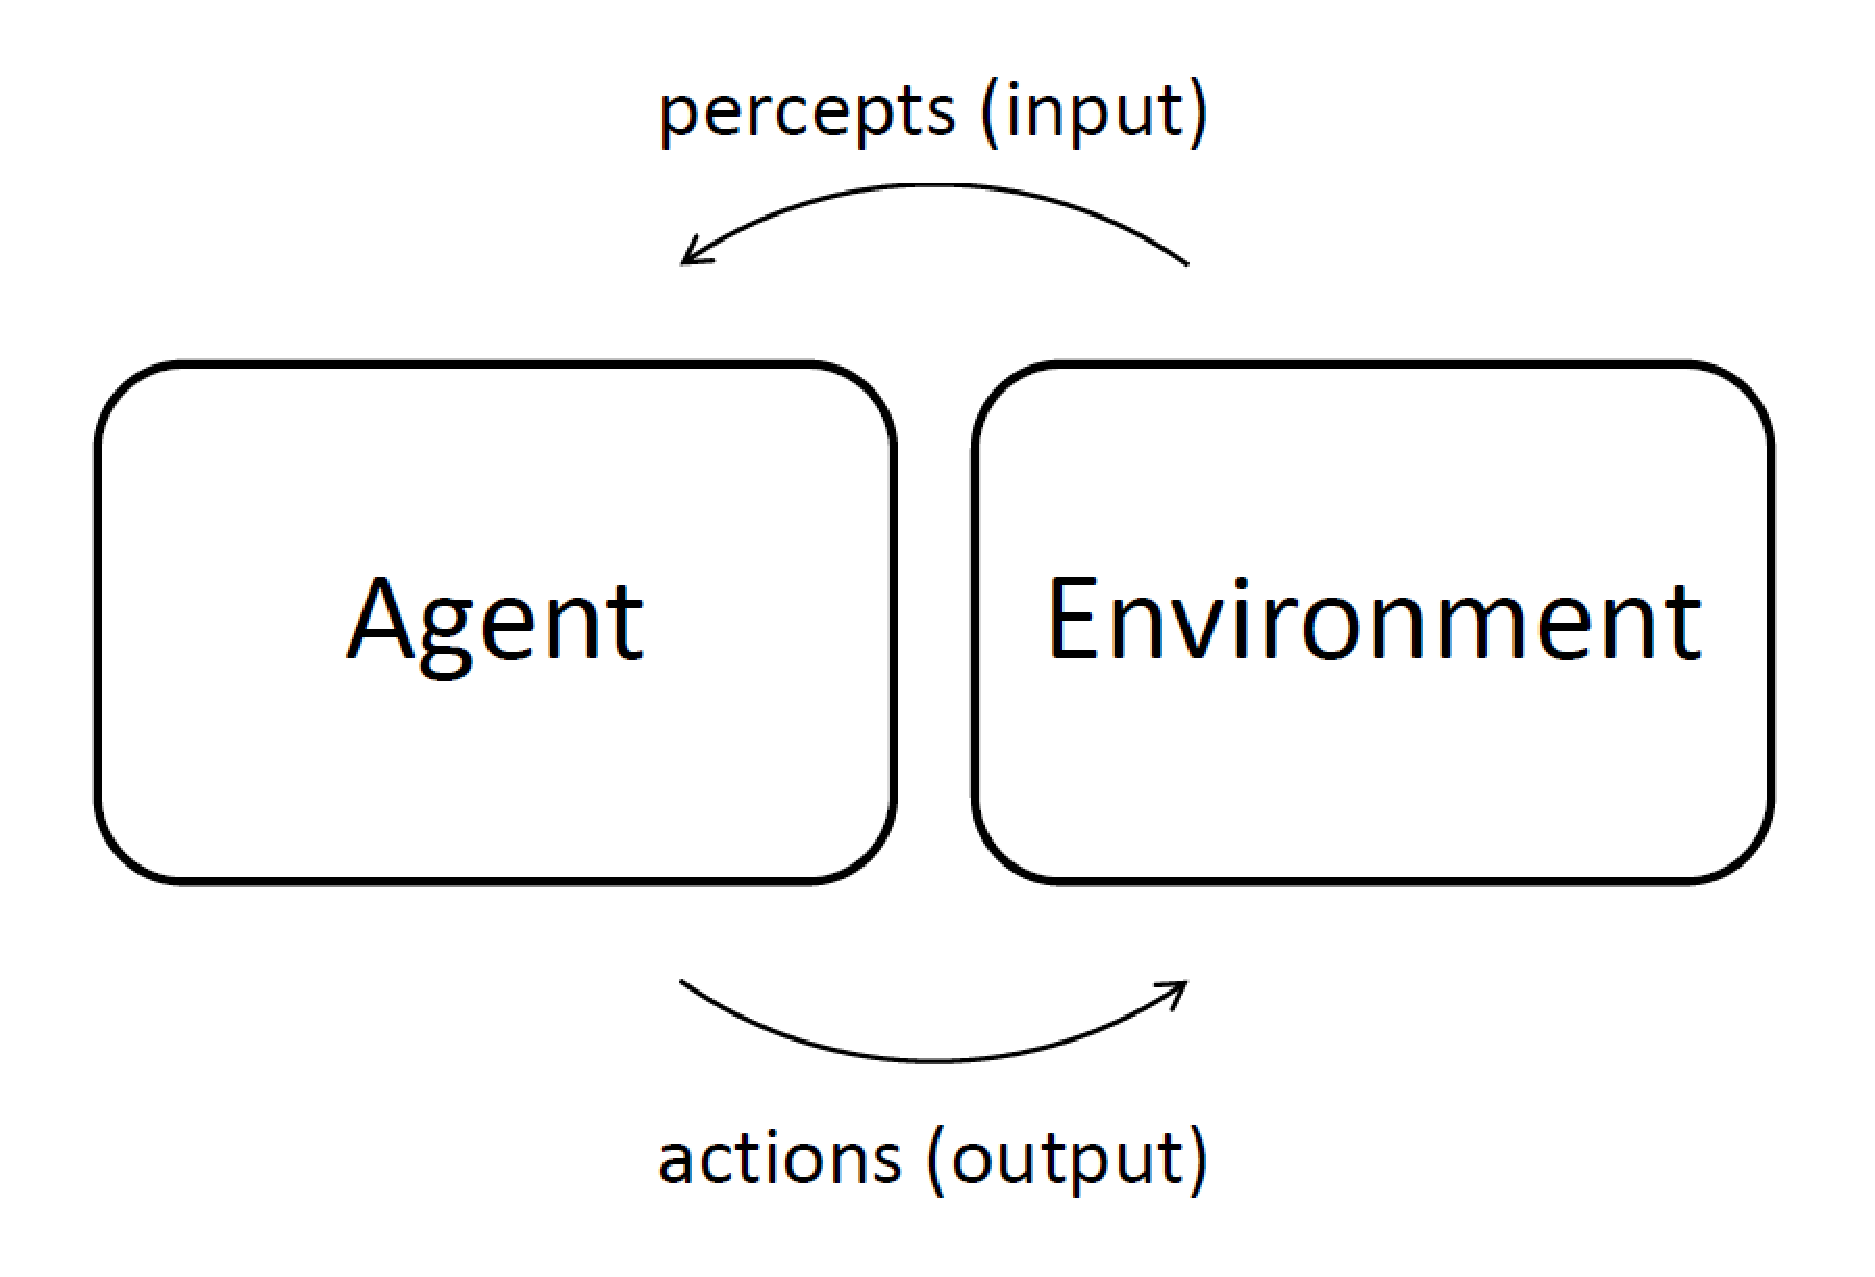
\includegraphics[width=0.4\textwidth]{images/agent-environment-interaction}
	\caption{An agent interacting with its environment}
	\label{figure:agent-environment-interaction}
\end{figure}

% Agent - example: softbot
An example of an agent is a \textit{softbot}---an agent situated in a software environment interacting with it via commands. A softbot's sensors are commands meant to provide information about the environment (e.g. \texttt{ls} or \texttt{pwd} in Unix) and its effectors are commands meant to change the environment (e.g. \texttt{mv} or \texttt{compress} in Unix).

%%%%%%%%%%%%%%%%%%%%%%%%%%%%%%%%%%%%%%%%%%%%%%%%%%%%%%%%%%%%%%%%%%%%%%%%%%%%%%%%
\section{Multi-Agent Systems}

% MAS slogan
There is a popular slogan in the multi-agent systems community: ``There's no such thing as a single agent system'' \cite{Wooldridge09}.

% MAS - definition
\textit{Multi-Agent system}\footnote{Alternatively spelled multiagent system.} (MAS) is a system composed of multiple interacting agents.

% MAS vs. single agent
Like a single agent,a MAS is situated in an environment, which means that all its constituent agents are situated in the same environment.
While the field of agents studies agents' interaction with their environment and their reasoning about it, the field of MASs deals with agents' interaction with other agents and their reasoning about them.
The inter-agent interaction can be either \textit{direct} (via messages) or \textit{indirect} (via environment).

% Empty environment
In this thesis, we do not consider agents' interaction with their environment and we do consider only direct inter-agent interaction---\textit{communication}.
Hence, we do not assume anything about the environment in which MASs are situated. In fact, as far as the discussion in this thesis goes, MASs do not have to be situated in any environment, i.e. situated in an \textit{empty} (non-perceivable, non-affectable) environment.

Most importantly, we do not assume any social structure of MASs; a MAS is really just a group of agents with no special relationships among them.
In other words, all agents are equal.
It is the aim of this thesis to introduce social structure to MASs.